\section{Analyse de la mobilité urbaine et interurbaine et cas particulier dans la ville de Yaoundé}

La mobilité urbaine et interurbaine a été et demeure toujours un sujet d'intérêt, un problème qui a toujours suscité l'attention, vu son importance dans le développement économique d'un État. Elle dépend fortement d'un ensemble de facteurs, lesquels facteurs retiendront notre attention dans l'analyse du cas de la ville de Yaoundé qui suit.

\subsection{Architecture routière de ville de Yaoundé}

\begin{figure}[h]
    \centering
    \includegraphics[width=0.5\linewidth]{Images/Reseau_Routier_Yaoundé.png}
    \caption{Réseau routier - Yaoundé}
    \label{fig:reseau_routier}
    \cite{mfoulou2016mobilite}
\end{figure}

Au vu de la carte \ref{fig:reseau_routier} ci-dessus, on constate que le réseau routier de la ville de Yaoundé a plus ou moins une structure en étoile, centrée au niveau du centre ville et principalement du lieu dit: poste centrale. 
C'est à juste titre (comme le montre l'illustration \ref{fig:trafic_routier} en dessous, qu'on observe un trafic intense au niveau des zones proches du centre ville.

\begin{figure}[h]
    \centering
    \includegraphics[width=0.72\linewidth]{Images/Traffic_Routier_Yaoundé.png}
    \caption{Trafic routier - Yaoundé}
    \label{fig:trafic_routier}
    \cite{mfoulou2016mobilite}
\end{figure}

On déplore alors cette architecture, qui favorise des embouteillages chroniques et très souvent des accidents.
Toutefois, un réseau routier basé sur plusieurs pôles au lieu d'un seul, aurait amélioré la situation.

\subsection{Évolution des modes de transports dans la ville de Yaoundé}

Les moyens de transports dans la ville de Yaoundé, ont fortement évolués depuis la crise économique dont a été victime le Cameroun dans les années 80. 

\subsection{La SOTUC et son déclin}

La SOTUC\footnote{Société des transports urbains du Cameroun.
} a été créée en 1973 pour assurer le transport public urbain à Yaoundé. \emph{A l'époque}, elle était le principal opérateur de transport avec une flotte de bus importante. Cependant, la SOTUC a connu un déclin progressif au fil des années. \emph{En 2023}, la société ne disposait que d'une centaine de bus en état de marche, ce qui est largement insuffisant pour répondre aux besoins de la population croissante de Yaoundé.

\subsection{L'émergence des motos-taxis}

Face à l'insuffisance de la SOTUC, les motos-taxis, communément appelées "clandos", ont fait leur apparition dans les années 1990. \emph{Elles sont rapidement devenues le mode de transport dominant à Yaoundé}, en raison de leur flexibilité et de leur coût abordable. On estime aujourd'hui qu'il y a plus de 200 000 motos-taxis en activité à Yaoundé.

Dès lors les déplacements dans la ville de Yaoundé se font exclusivement via les taxis en plein coeur de la ville, et via les motos pour les coins reculés et les quartiers périphériques.

\subsection{État actuel de la mobilité dans la ville de Yaoundé}

\begin{figure}[h]
    \centering
    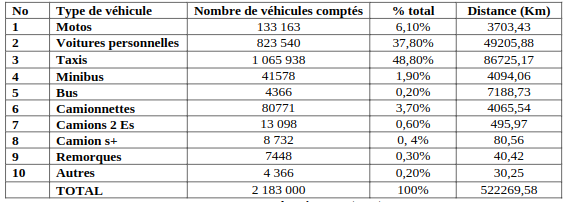
\includegraphics[width=0.8\linewidth]{Images/Repartition_Trafic_Par_Vehicule.png}
    \caption{Répartition du trafic routier à Yaoundé}
    \label{fig:repartition_trafic}
    \cite{mfoulou2016mobilite}
\end{figure}

Les statistiques sont claires. Les citoyens de la ville de Yaoundé se déplace exclusivement en taxi
 ou en moto. Les facteurs déterminants pour le choix de mobilité à Yaoundé incluent l’accessibilité, la densité de la zone d’origine, et le motif de déplacement. L’accessibilité influence négativement l’usage de la moto et du taxi, mais positivement celui du bus, minibus et voiture personnelle. Les zones denses encouragent l’usage de la moto en raison de l’absence d’aménagements publics et de la demande élevée en mobilité, tandis que la densité a un impact négatif sur le choix du taxi dû à la congestion. Le motif de déplacement influence positivement tous les modes de transport, avec une préférence moindre pour la moto pour se rendre au travail. La localisation du logement par rapport aux grands axes radiaux et la distance du goudron sont également cruciales, tandis que l’heure de déplacement n’affecte pas l’usage de la moto ou de la voiture personnelle.

 Mais quelles peuvent être les conséquences de ces choix de mobilité ?

 \subsection{Problèmes de mobilité dans la ville de Yaoundé}

Vu la structure centrée de la ville de Yaoundé et de l'usage exclusif de moyens de transports à faible capacité (taxis et motos), celle-ci est très fréquemment le théâtre de congestion et de difficultés de déplacements, ce qui est un problème qui prend de plus en plus de l'ampleur. D'autant plus que l'usage des bus (plus appropriés pour résoudre le problème), ne se ressent quasiment plus.

Face à une ville avec une structure inadéquate pour les transports de masse, et très souvent aussi à l'incivisme des conducteurs d'automobile, une plate-forme accessible à tous, qui permettrait de repartir de manière uniforme le trafic dans la ville s'avère alors utile.,Mais alors, quelles fonctionnalités devrait avoir une telle solution en vue de résoudre optimalement le problème posé, et en vue de mieux s'intégrer dans la vie de tous les jours ? C'est ce dont nous en parlerons dans la suite 




